\section{Yao's Garbled Circuits}

In oblivious transfer, the function 
$f$ can be transformed into a Boolean 
circuit (possible for all polynomial 
time functions) and represented as 
a directed acyclic graph using only 
AND and XOR gates for the nodes and 
boolean valued wires for the edges. 

Assign one encryption key for every 
possible boolean value on wires.
“Double encrypt” output keys with 
corresponding input keys.
\begin{figure}
    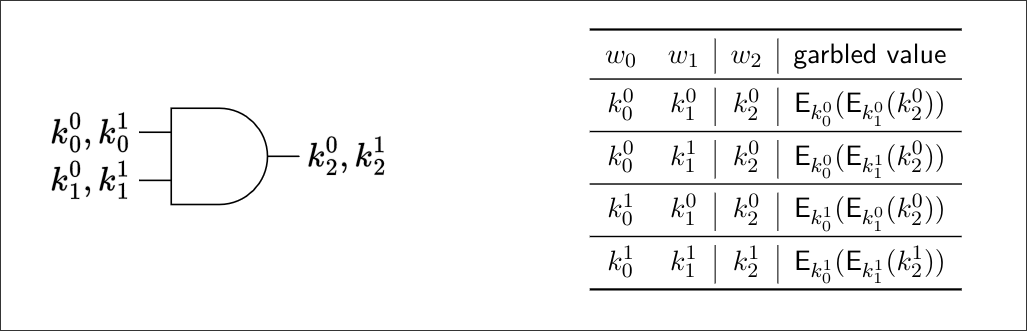
\includegraphics[width=\textwidth]{images/1.png}
\end{figure}

A garbled gate consists of the doubly 
encrypted output key values.
\begin{figure}
    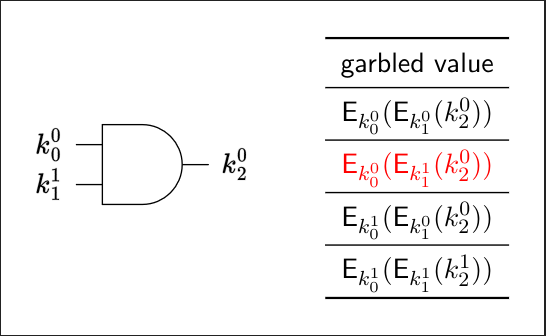
\includegraphics[width=\textwidth]{images/2.png}
\end{figure}
How do we evaluate a garbled gate?
Using keys corresponding to input values: $k_0^0$,
$k_1^1$ (corresponding to 01 input).
Note that key values don't reveal anything about 
the actual wire Boolean value.
We can give input keys to a party and ask 
them to evaluate the gate; but
they can obtain the output key without 
learning the wire values on input/output.
We need to randomly permute rows (and use 
encryption with wrong key detection).
\begin{figure}
    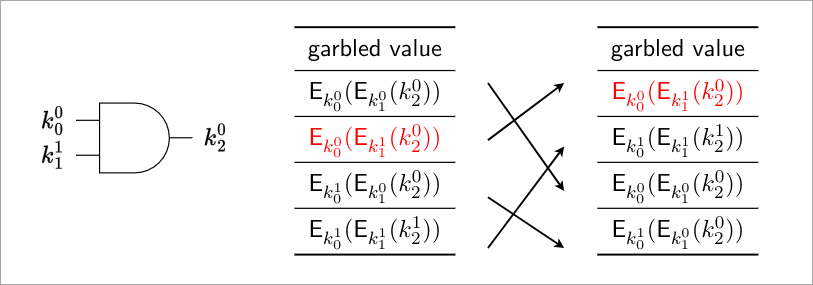
\includegraphics[width=\textwidth]{images/3.png}
\end{figure}